% !TEX root = thesis-thomas-tiotto.tex

\section{Data set} \label{sec:data-set}
As anticipated in Chap. \ref{chap:introduction} the work carried out in this thesis had a certain degree of collaboration with a third party, \cite{istitutocantonalepresentazione}.

\subsection{Istituto Cantonale di Patologia}
Istituto Cantonale di Patologia (ICP) is an institute based in Locarno that is specialised in the histological analysis of tissue samples received from private patients, clinics and hospitals, mainly in support of cancer diagnosis.
Its Laboratory of Medical Diagnostics supports pathologists in the diagnosis of neoplastic diseases through the application of cytogenetic techniques; that is, the focus is on understanding how chromosomes relate to cell behaviour, particularly during mitosis and meiosis.
One of the techniques used is Fluorescence in Situ Hybridization (FISH) that is able to localise the presence or absence of specific DNA sequences in chromosomes.
These tests are aimed at identifying the precise profile of the cancer cells and thus inform the clinician on the best treatment for the specific patient.

In addition to its clinical support activities, the Istituto also carries out scientific research aimed at better understanding certain types of cancers at a basic level.
In the last ten years, the ICP has published more than 200 peer-reviewed papers and more than 100 works in non-peer reviewed journals and is active at a national and international level.

\subsection{Motivation}
My first contact with the ICP was during a meeting with Dr. Vittoria Martin (\cite{martin2012}), molecular citogenetist, in date 28/01/2019.
The institute had expressed interest in bringing machine learning into their workflow in order to both augment their profiling capabilities for patients and to be able to extract new knowledge from their existing data.
This knowledge-extraction may lead towards the confirmation of current scientific theories or may be the first step towards the formulation of novel ones.

\todo[inline]{chiedere a Vittoria cosa si aspettavano/aspettano}

My interest in collaborating with the Istituto stemmed from the desire to apply the methods described in Sec. \ref{sec:novel-contributions} to a real-world case.
Being the theoretical work being carried out in this thesis an expert-driven MPE approximation, collaboration with the institute has also provided the opportunity to implement a proof of concept using real histological data.
The doctors and researchers of the Istituto have been able to validate, from an Explainable AI and clinical relevance points of view, the model software that I have developed.
That is to say, they have validated the capacity of the developed software both in its capacity to support clinical decision making and to surface clarifying explanations of the data set and in its adherence to established medical literature.

\todo[inline]{da confermare con Vittoria piu avanti}

\subsection{Provided Data Set}
The data set I was provided with was created by \textit{Registro Tumori Ticino} (Locarno, Ticino) in order to highlight possible new relations between clinical, histopathological and molecular features, as well as to potentially discover novel biomarkers for the progression of the disease 
It consists of the histological records over 38 recorded variables of 3218 breast cancer patients who have been diagnosed between the years 2005 and 2014 within the Ticino canton of Switzerland.
The data set had been pre-processed by collaborators of IDSIA in agreement with the ICT with 13 of the variables being dropped, because not considered relevant.
In particular, all variables relating to the patient post-treatment were discarded as well as those recording the diagnosis date.
In Tab. \ref{tab:datasetvariables} is a description of the measured variables, together with their clinical meaning.
The value distribution of the data set is shown in Tab. \ref{tab:datasetdistribution}.

The indications from Dr. Martin on how to further preprocess the data are shown in Tab. \ref{tab:datasetpreprocess}.
Note that some variable names were simplified.

\begin{table*}[htbp]
\caption{Data set variables}
\begin{tabularx}{\textwidth}{@{} l Y @{}}
\toprule 
\textbf{Variable} & Clinical meaning \\
\midrule 
\textbf{Codice globale} & Unique patient identifier \\
\textbf{mut17q21} & Mutation of chromosome 17 \\
\textbf{loss 17} & Loss of chromosome 17 \\
\textbf{et\`a arrotondata} & The age of the patient at diagnosis \\
\textbf{Lateralit\`a} & The affected breast \\
\textbf{Situ SUBGROUP MZ} & The primary site code of the tumour \\
\textbf{Morfologia SUBGROUP MZ} & The morphology classification of the tumour \\
\textbf{pT SUBGROUP MZ} & Primary tumour in the TNM classification for breast cancer \\
\textbf{pN SUBGROUP MZ} & Pathologic in the TNM classification for breast cancer \\
\textbf{M 8.2.96} & Distant metastasis in the TNM classification for breast cancer \\
\textbf{Differenziazione} & Tumour grade \\
\textbf{Recettori estrogeni percento 1.1.2003} & Expression of estrogen receptors \\
\textbf{Recettori progestinici percento 1.1.2003} & Expression of progestin receptors \\
\textbf{c erbB 2  cod percento 1.1.2003} & ErbB2 marker expression \\
\textbf{Ki67 cod percento} & Tumoural proliferation index \\
\textbf{FISHRatio} & FISH analysis result \\
\bottomrule
\end{tabularx}
\label{tab:datasetvariables}
\end{table*}

\begin{table*}[htbp]
\caption{Data set distribution before pre-processing}
\begin{tabularx}{\textwidth}{@{} l X c @{}}
\toprule 
\textbf{Variable} & Unique values & Distribution \\
\midrule 
\textbf{mut17q21} & 2 & 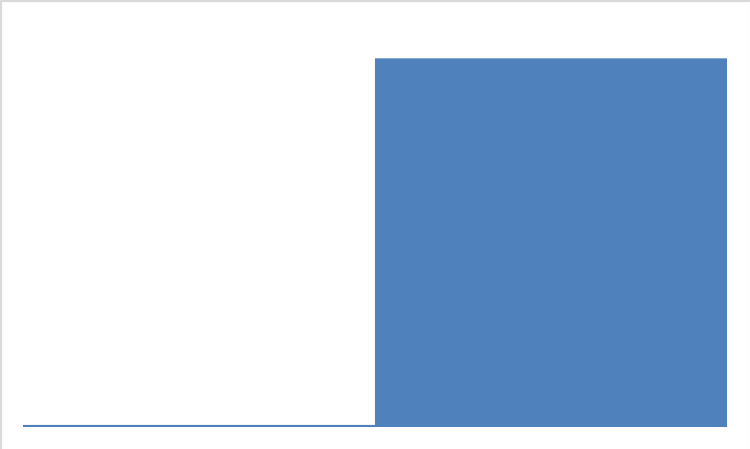
\includegraphics[width=0.2\textwidth, height=10mm]{methodology/images/mut17q21}  \\
\textbf{loss 17} & 3 & 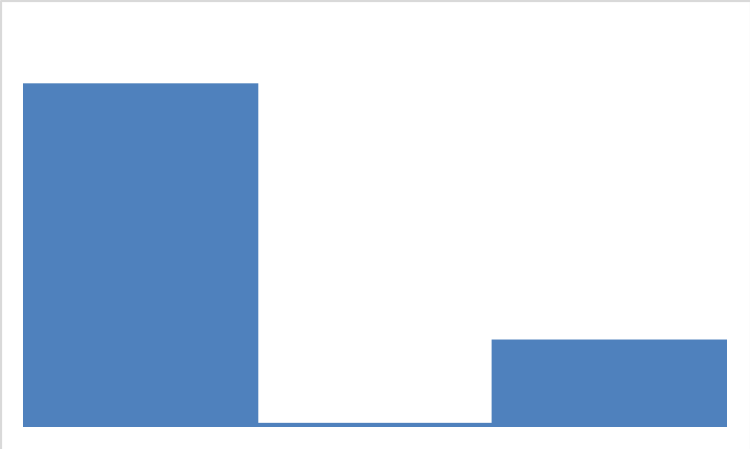
\includegraphics[width=0.2\textwidth, height=10mm]{methodology/images/loss_17}\\
\textbf{eta arrotondata} & 74 & 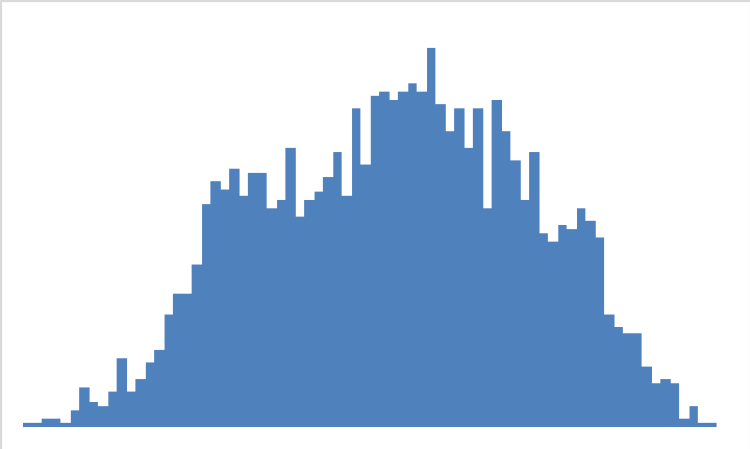
\includegraphics[width=0.2\textwidth, height=10mm]{methodology/images/eta_arrotondata}\\
\textbf{ateralit\`a} & 3 & 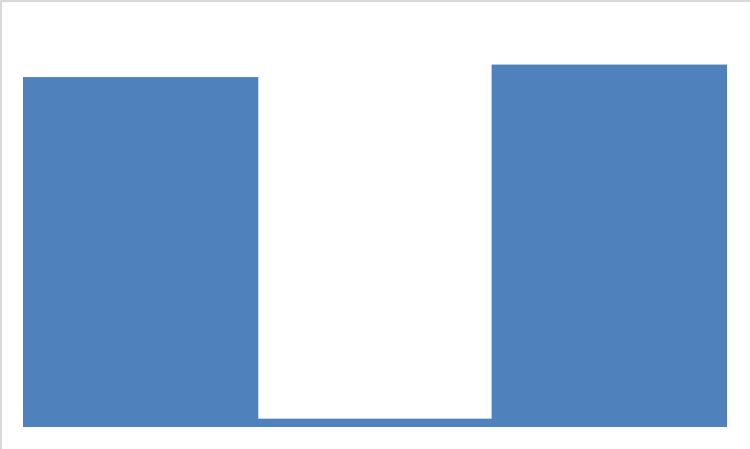
\includegraphics[width=0.2\textwidth, height=10mm]{methodology/images/lateralita} \\
\textbf{situ} & 5 & 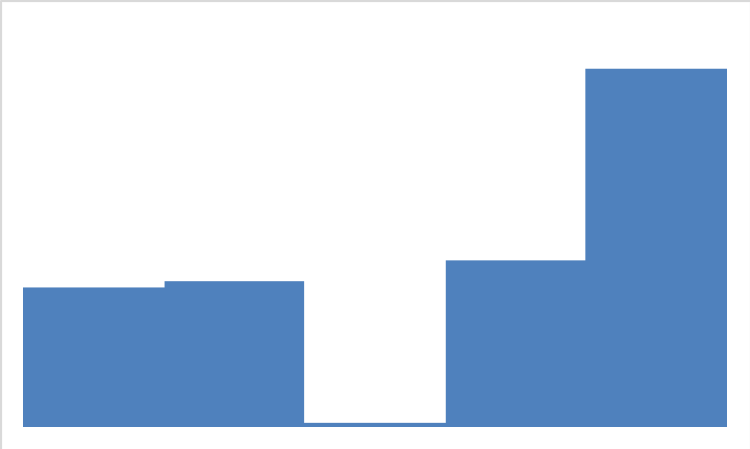
\includegraphics[width=0.2\textwidth, height=10mm]{methodology/images/situ} \\
\textbf{morfologia} & 5 & 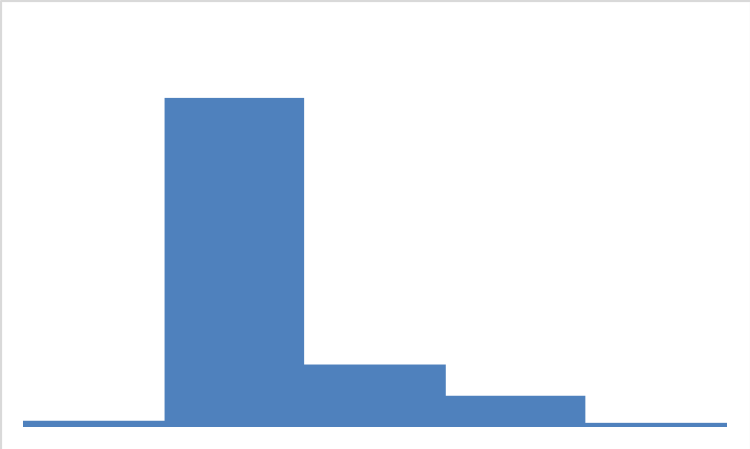
\includegraphics[width=0.2\textwidth, height=10mm]{methodology/images/morfologia} \\
\textbf{pT} & 23 & 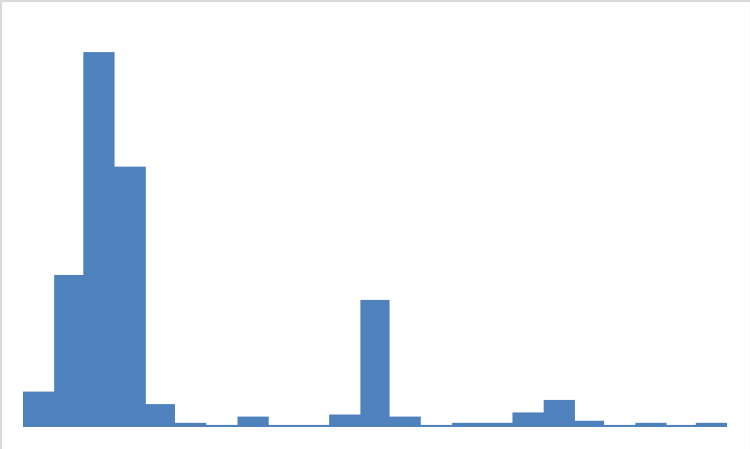
\includegraphics[width=0.2\textwidth, height=10mm]{methodology/images/pt} \\
\textbf{pN} & 6 & 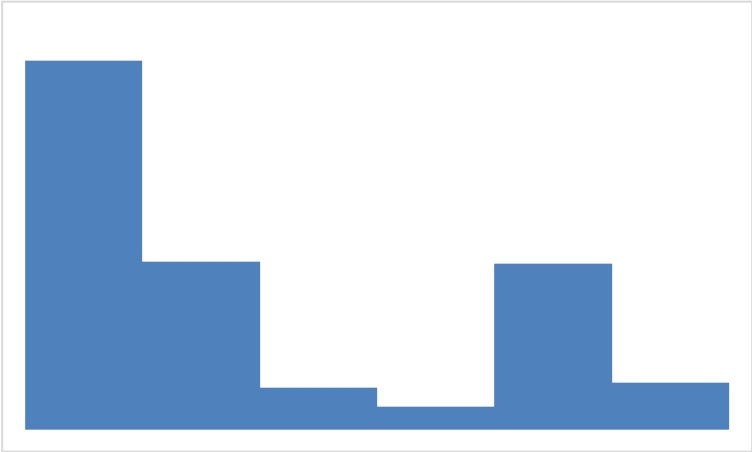
\includegraphics[width=0.2\textwidth, height=10mm]{methodology/images/pn} \\
\textbf{M} & 3 & 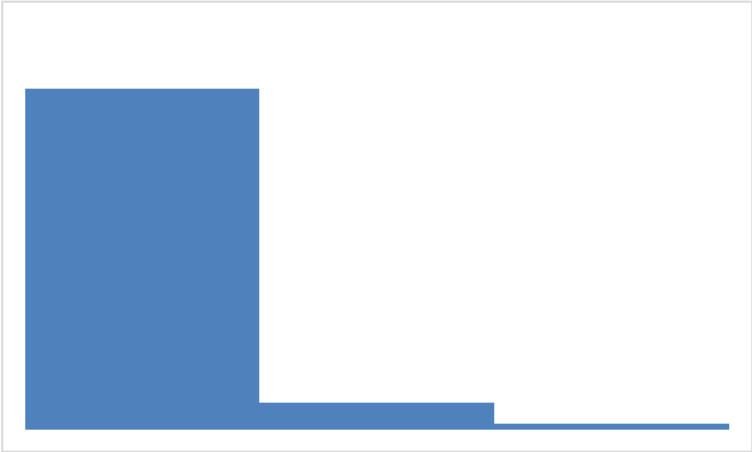
\includegraphics[width=0.2\textwidth, height=10mm]{methodology/images/m} \\
\textbf{differenziazione} & 5 & 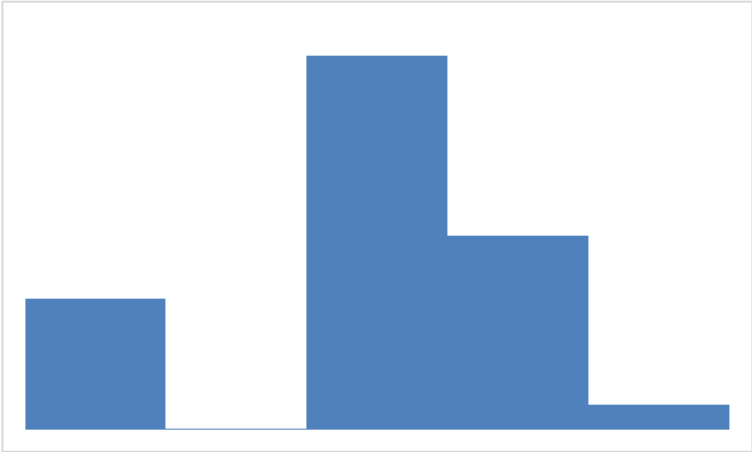
\includegraphics[width=0.2\textwidth, height=10mm]{methodology/images/differenziazione}  \\
\textbf{recettori estrogeni} & 40 & 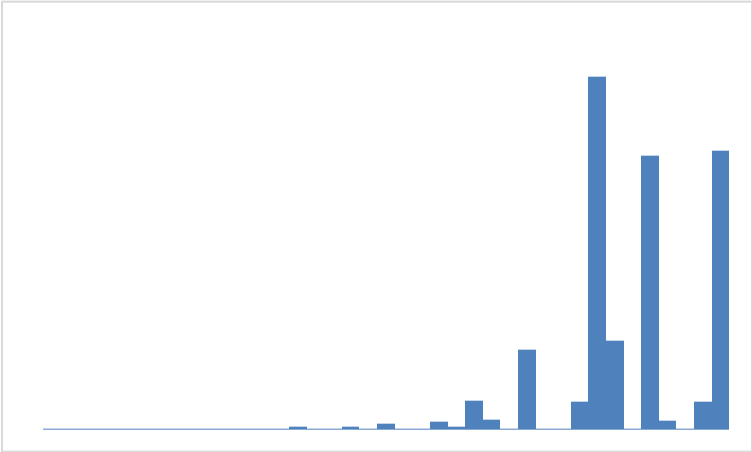
\includegraphics[width=0.2\textwidth, height=10mm]{methodology/images/recettori_estrogeni} \\
\textbf{recettori progestinici} & 40 & 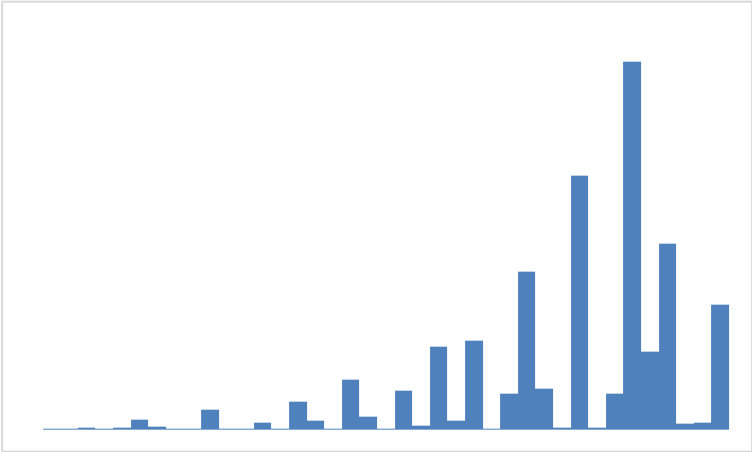
\includegraphics[width=0.2\textwidth, height=10mm]{methodology/images/recettori_progestinici}\\
\textbf{c erbB 2} & 4 & 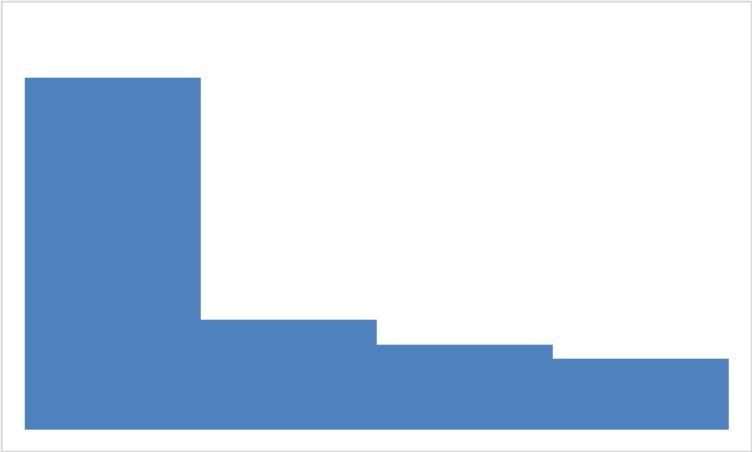
\includegraphics[width=0.2\textwidth, height=10mm]{methodology/images/c_erb_2}\\
\textbf{Ki67} & 52 & 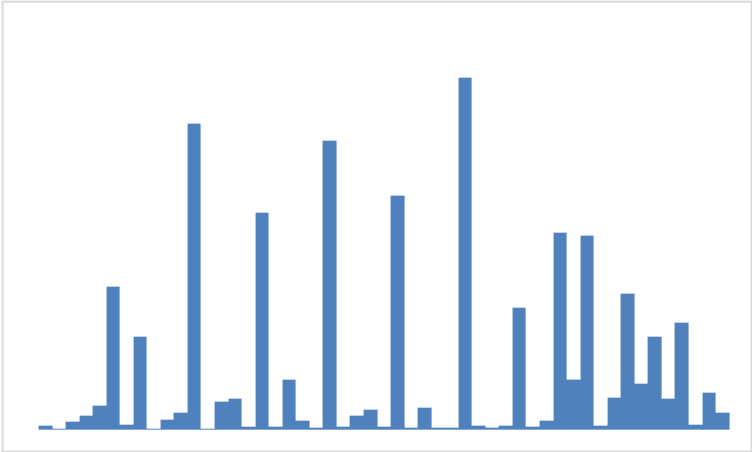
\includegraphics[width=0.2\textwidth, height=10mm]{methodology/images/ki67}\\
\textbf{FISH} & 5 & 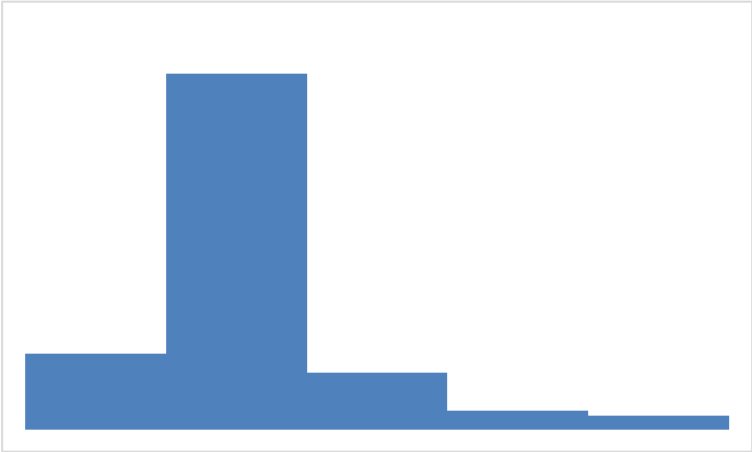
\includegraphics[width=0.2\textwidth, height=10mm]{methodology/images/fish}\\
\bottomrule
\end{tabularx}
\label{tab:datasetdistribution}
\end{table*}

\begin{table*}[htbp]
\caption{Data set preprocessing steps}
\begin{tabularx}{\textwidth}{@{} l Y @{}}
\toprule 
\textbf{Variable} & Action \\
\midrule 
\textbf{Codice globale} & Remove variable \\
\textbf{mut17q21} & Remove blanks \\
\textbf{loss 17} & Remove blanks \\
\textbf{eta arrotondata} & Bin into \enquote{$< 40$}, \enquote{$40-50$}, \enquote{$\geq 50$} \\
\textbf{lateralita} & Remove blanks and \enquote{sconosciuta} \\
\textbf{situ} & Remove blanks \\ \addlinespace
\textbf{morfologia} & Remove blanks and \enquote{unuseful} if performance on classification is subpar \\ \addlinespace
\textbf{pT} & Remove blanks and \enquote{unuseful}  \\
\textbf{pN} & Remove blanks and bin into \enquote{0} and \enquote{$\neq0$}\\
\textbf{M} & Remove blanks \\ 
\textbf{differenziazione} & Remove blanks and \enquote{Sconosciuto o non applicabile} \\ \addlinespace
\textbf{recettori estrogeni} & Remove blanks and bin into \enquote{negativo} if $\leq 10$,
		\enquote{debolmente positivo} if $\leq 50$, 
		\enquote{fortemente positivo} if $> 50$ \\ \addlinespace
\textbf{recettori progestinici} & Remove blanks and bin into \enquote{negativo} if $\leq 10$, 
		\enquote{debolmente positivo} if $\leq 50$, 
		\enquote{fortemente positivo} if $> 50$ \\ \addlinespace
\textbf{c erbB 2} & Remove blanks \\ 
\textbf{ki67} & Remove blanks and bin into \enquote{<14}, 
		\enquote{14-20}, \enquote{20-30}, \enquote{>30} \\ 
\textbf{FISH} & Remove blanks \\
\bottomrule
\end{tabularx}
\label{tab:datasetpreprocess}
\end{table*}

\section{Validation Methodology}
\todo[inline]{discutere con Vittoria come validare al meglio}
Having direct access to expert pathologists has not only helped in guiding research into the theoretical explainability properties of the system but also enabled their validation.
There are two main validation streams to be addressed: from the clinical point of view and from the explainability one, with the results of the latter depending on those of the former.
 
\subsection{Clinical validation}
A validation of the methods carried out in this thesis in their adherence to established clinical literature, is of paramount importance.
A failure on the Bayesian Network's part in capturing the true relationships between the variables would hamper it in being able to give any meaningful representation of them.
For the expert to even start to trust the system or to be able to make sense of its outputs, it is vital that there be as little cognitive dissonance between the experts' basic beliefs and expectations and those that he sees represented in the system.

For this reason, the initial validation phase with the Istituto Cantonale di Patologia concentrated on the clinical validation aspect.
The methodology chosen to clinically validate the system was for a representative of the ICT to formulate a series of natural language queries; each one of these was annotated with the specific queried variable in the network and its value together with the known values of other variables.
The ICT's delegate included the expected reply to the queries together with its probability, based on the latest medical literature and their personal expertise.
So, each query asked for the probability truth value of the following:
\begin{align}
	(var_1 = a \wedge \ldots \wedge var_n = z ) \Rightarrow var_k = k \quad var_1 \ldots var_n \in V, var_k \in V \smallsetminus \{ var_1 \ldots var_n \}
\end{align}
This would translate into natural language into:
\enquote{If $var_1$ is $a$ and $\ldots$ and $var_n$ is $z$, how probable is it that $var_k$ $k$?}.
The complete series of eight questions, together with the expected values, is shown in Tab. \ref{tab:clinicalvalidationquestions}.
It is quite evident that all these validation questions are instances of the Bayesian Network Updating problem, in particular they are Conditional Probability Queries (as defined in \ref{subsec:bnupdating}).

\todo{inserire tabella qui o in Results}

\subsection{Explainability validation} \label{subsec:explainability-validation}
Having validated the system in terms of its adherence to clinical literature, it could then also meaningfully be validated from an explainability point of view.
The main question to be addressed is its capacity to relate to the expert user.
Is the system able to engender the user's trust?
In doing so, is she able to extract more knowledge from existing data when using the system than not?
Especially in cases where there may be a dearth of data, can the expert maximise the benefit from the available information?
Does the user subjectively feel that the system may positively impact her work?
These are all hard questions to answer, as there is a very high degree of subjectivity involved.
Thus to attempt to answer them, the chosen methods were borrowed from the social sciences.

In an earlier stage, the experts were introduced to the system in prototype form and instructed on the possible use cases it offered.
Then, they were asked to keep track of times they felt they could have used the system, had it been available, during their day-to-day work and to report back to me with the query they would have submitted to the system.
If the query were in the realm of possibilities offered by my program, I would submit the outputs back to the users together with the following questionnaire:
\todo[inline]{definire questionario da mandare con le domande}
This process would both give feedback on the performance of the system and also inform its design.

In a later phase, having finalised the system's design, I provided it to the experts at the ICT for their use in their daily work.
After \textbf{xx time} I followed up with them with an interview based on the following format:
\todo[inline]{definire formato e metriche intervista}
This enabled me to quantify the performance of the system, as perceived by its users in a real setting, over an extended period of time.

